\documentclass[a4paper,12pt]{article}
\usepackage{graphicx} % This package is used to allow us to include a
                      % wide range of graphics formats within the
                      % document.  We can add many different packages
                      % with LaTeX, but for most purposes, a small
                      % subset is sufficient.
\begin{document}

Hello world! What chance is there of this working?

\section{Quick start example}
\label{mystart} % Note that the percent character is used for comments - everything that follows on the same line is ignored.
You have to begin somewhere.  This trivial example shows you how to
write some mathematics, which is one of the most obvious differences compared to using e.g. MS Word and Equation Editor.  Maths can be written "inline" or displayed separately from the paragraph text, either as a numbered or an unnumbered equation.
For example,  typing
\verb=$\Lambda_b\to\Lambda^0\mu^+\mu^-$= will produce
$\Lambda_b\to\Lambda^0\mu^+\mu^- $ (the \$ symbol tells LaTeX to start
formatting what follows as mathematics, the trailing \$ to stop this
formatting.

If you want to write your maths as a separate numbered equation, you use a simple syntax like
\begin{verbatim}
\begin{equation}
A=b+c
\label{trivial}
\end{equation}
\end{verbatim}

which is displayed as 
\begin{equation}
A=b+c
\label{trivial}
\end{equation}

Note that LaTeX does not care about whitespace between words in a paragraph, it sorts out the interword spacing for you.  To start a new paragraph, simply leave a blank line in your input file. 


\subsection{Equations}
\label{my_subsection}
With a little more substance, and interest, we introduce

% The \begin{verbatim} denotes that everything to follow will *not*
% be processed as commands by latex, will simply
% appear on the page exactly as below, including spaces.
\begin{verbatim}
\begin{equation}
\sigma(e^+ e^- \rightarrow f\overline{f})
  = \frac{12\pi}{m^2_Z}
  \frac{s\Gamma_\mathrm{e}\Gamma_f}{(s-m^2_Z)^2+\Gamma^2_Zm^2_Z}
\label{rbw}
\end{equation}
\end{verbatim} % This denotes the end of the ``verbatim'' section.
which when formatted by LaTeX, appears as 
\begin{equation}
\sigma(e^+ e^- \rightarrow f\overline{f})
  = \frac{12\pi}{m^2_Z}
  \frac{s\Gamma_\mathrm{e}\Gamma_f}{(s-m^2_Z)^2+\Gamma^2_Zm^2_Z},
\label{rbw}
\end{equation}

You can refer to objects such as equations, tables, subsections,
etc. by using the \verb+\ref+ command, e.g.
\begin{verbatim}
See equation~\ref{trivial} and equation~\ref{rbw}
\end{verbatim}
 is typeset as ``See equation~\ref{trivial} and equation~\ref{rbw}".

\subsection{References}
 Similarly, you can refer to subsections (or any other object) in
 the same way, by adding a \verb+\label{mytext}+ directly after
 the element you are interested in, and then referring to it
 using \verb+\ref{mytext}+.  The numbering for each set of
 elements such as tables, figures, equations is independent.

 For example, we can refer to Section~\ref{my_subsection},
 Section~\ref{mystart}, Equations~\ref{trivial} and \ref{rbw}, and the
 equation found on page~\pageref{rbw} using the following:

\begin{verbatim}
 Section~\ref{mystart}, Equations~\ref{trivial} and \ref{rbw}, and the
 equation found on page~\pageref{rbw}
\end{verbatim}

There are many aspects of using LaTeX that will save you time, see online tutorials for examples.
You can make lists using several different constuctions, e.g.
\begin{verbatim}
\begin{itemize}
 \item first
 \item second
\end{itemize}
or 
\begin{enumerate}
 \item firstly
 \item secondly
\end{enumerate}
and lists can of course be nested, 
\begin{enumerate}
 \item first
 \item second
 \begin{enumerate}
  \item firstly
  \item secondly
 \end{enumerate}
\end{enumerate}
\end{verbatim}

 The above is formatted as
\begin{itemize}
 \item first
 \item second
\end{itemize}
or 
\begin{enumerate}
 \item firstly
 \item secondly
\end{enumerate}
and lists can of course be nested, 
\begin{enumerate}
 \item first
 \item second
 \begin{enumerate}
  \item firstly
  \item secondly
 \end{enumerate}
\end{enumerate}

Note that in this example, we have not worried about how the nested
levels of list are formatted, we have only told LaTeX that the lists
are inside one another.  Whether the different levels are formatted as
2(a) or 2(1) or 2(i), etc. is only a detail of appearance.  This can
of course be changed within your document, but such changes are
normally made for the whole document, to maintain uniform appearance,
as you would when writing a textbook or scientific paper.

\subsection{Including images}
Images can be included in most graphics formats (.pdf, .png, .jpg,
.eps, ...), but not all types can be mixed within the same document
(notably .eps and others).

The usual way to include a figure is within a \verb+\begin{figure}...+
environment.

\begin{verbatim}
% The "optional" arguments appear in square brackets define position of
% the figure within the document: "here"; "top", "bottom" (of page),
% or (separate) "page".
\begin{figure}[htbp]
  \centering
  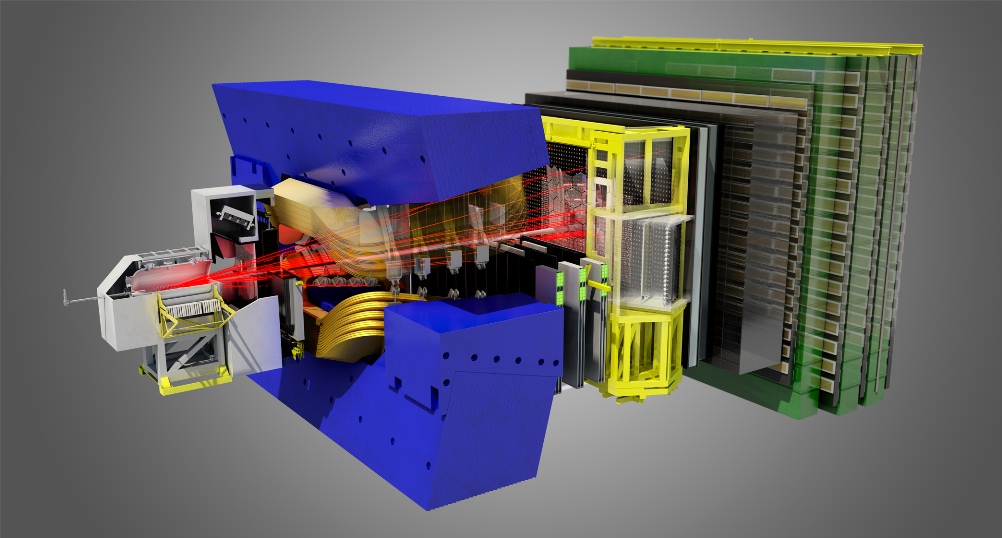
\includegraphics[width=0.8\textwidth]{LHCbDetectorpnglight1.png}
\caption{Here is one we made earlier}
\label{mydetector}
\end{figure}
\end{verbatim}
\begin{figure}
% The "optional" arguments appear in square brackets define position of
% the figure within the document: "here"; "top", "bottom" (of page),
% or (separate) "page".
  \centering
  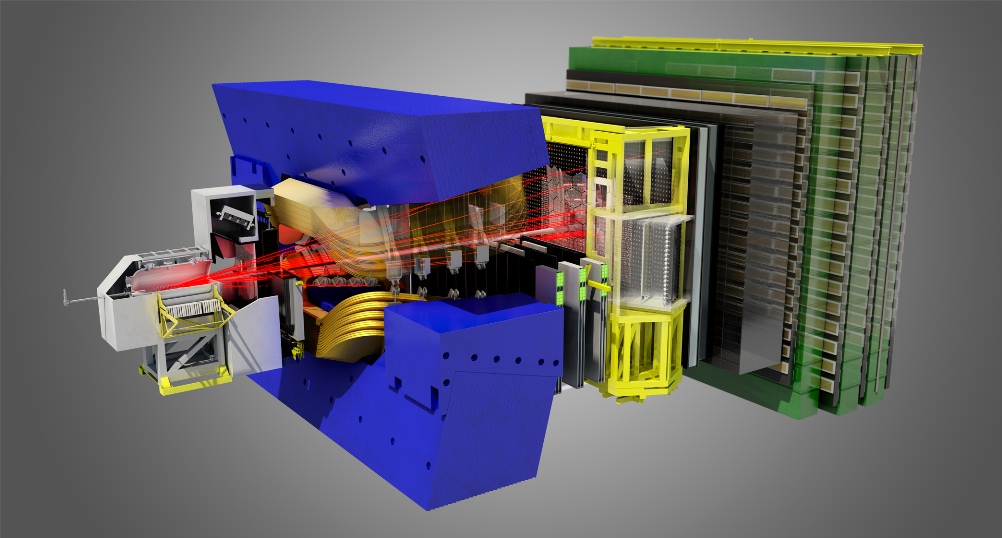
\includegraphics[width=0.8\textwidth]{LHCbDetectorpnglight1.png}
  \caption{Here is one we made earlier}
  \label{mydetector}
\end{figure}

We refer to the figure as
\verb+Figure~\ref{mydetector}+ which formats as
Figure~\ref{mydetector}. (Note that the \verb+~+
character which we keep using is invisible ``glue'' character, by
default it is not formatted, but ensures two characters are not
separated from each other, hence often used to tie an object such as
Figure, Table, Section to its related number.

\subsection{Footnotes and citations}
LaTeX makes it easy to use footnotes\footnote{Excessive use is
  distracting.}, but you can insert them trivially and not worry about
where they will appear in the text.  This footnote is created using
\begin{verbatim}
...to use footnotes\footnote{Excessive use is distracting.}, but you ...
\end{verbatim}

Similarly, using a bibliography is straightforward. In its simplest
form, and this is the best way to get started, you can define your own
format for references in the same source document as you are
preparing your main text.  This is very efficient for up to
medium-sized documents.  When you repeatedly write about similar
subjects, you may prefer to create a LaTeX database (usually with the
\verb+bibtex+ package) which, although it can be slower to set up
initially, will save time overall.  It can be particularly useful for
larger collaborative projects (think: Group Studies).  Furthermore,
there are many online databases of publications that can create the
required LaTeX (or bibtex) output for you directly.  You can refer to
your favourite set of papers used in your document, which may include
a more-or-less well-known paper~\cite{Higgs:1964pj} from 1964, which was
followed by a related pair of articles~\cite{Higgs:1964ia,Higgs:1966ev}.

Each of these citations is generated using the commands, e.g.
\begin{verbatim}
well-known paper~\cite{Higgs:1964pj}...
pair of articles~\cite{Higgs:1964ia,Higgs:1966ev}}.
\end{verbatim}
where the argument of the \verb+\cite+ command must match the
corresponding \verb+\bibitem{...}+ element in the bibliography part of
your source(s) file(s).

The format of the bibliograhy consists of a
\verb+\begin{thebibliography}+, a \verb+\end{thebibliography}+, and a
series of \verb+\bibitem{mytext}+ entries, one per reference to be
cited. The format of each of these \verb+\bibitem{mytext}+ entries is
free for you to choose, but you may wish to follow a style, e.g. as
used in a particular scientific journal related to your particular
field of interest.

The bibliography used in this example is generated using the following
LaTeX source commands:
\begin{verbatim}
\begin{thebibliography}{99} % The 99 here just means that the list of
                            % references can be up to 2 characters in
                            % length, so 99 maximum references.
%\cite{Higgs:1964pj}
\bibitem{Higgs:1964pj}
  P.~W.~Higgs,
  %``Broken Symmetries and the Masses of Gauge Bosons,''
  Phys.\ Rev.\ Lett.\  {\bf 13} (1964) 508.
  %%CITATION = PRLTA,13,508;%%
  %2857 citations counted in INSPIRE as of 06 Oct 2014

%\cite{Higgs:1964ia}
\bibitem{Higgs:1964ia}
  P.~W.~Higgs,
  %``Broken symmetries, massless particles and gauge fields,''
  Phys.\ Lett.\  {\bf 12} (1964) 132.
  %%CITATION = PHLTA,12,132;%%
  %2852 citations counted in INSPIRE as of 06 Oct 2014

%\cite{Higgs:1966ev}
\bibitem{Higgs:1966ev}
  P.~W.~Higgs,
  %``Spontaneous Symmetry Breakdown without Massless Bosons,''
  Phys.\ Rev.\  {\bf 145} (1966) 1156.
  %%CITATION = PHRVA,145,1156;%%
  %2076 citations counted in INSPIRE as of 06 Oct 2014
\end{thebibliography}
\end{verbatim}

\begin{thebibliography}{99} % The 99 here just means that the list of
                            % references can be up to 2 characters in
                            % length, so 99 maximum references.

%\cite{Higgs:1964pj}
\bibitem{Higgs:1964pj}
  P.~W.~Higgs,
  %``Broken Symmetries and the Masses of Gauge Bosons,''
  Phys.\ Rev.\ Lett.\  {\bf 13} (1964) 508.
  %%CITATION = PRLTA,13,508;%%
  %2857 citations counted in INSPIRE as of 06 Oct 2014

%\cite{Higgs:1964ia}
\bibitem{Higgs:1964ia}
  P.~W.~Higgs,
  %``Broken symmetries, massless particles and gauge fields,''
  Phys.\ Lett.\  {\bf 12} (1964) 132.
  %%CITATION = PHLTA,12,132;%%
  %2852 citations counted in INSPIRE as of 06 Oct 2014

%\cite{Higgs:1966ev}
\bibitem{Higgs:1966ev}
  P.~W.~Higgs,
  %``Spontaneous Symmetry Breakdown without Massless Bosons,''
  Phys.\ Rev.\  {\bf 145} (1966) 1156.
  %%CITATION = PHRVA,145,1156;%%
  %2076 citations counted in INSPIRE as of 06 Oct 2014
\end{thebibliography}

\end{document}
